\documentclass[conference]{IEEEtran}
\IEEEoverridecommandlockouts

\usepackage{iftex}
\ifXeTeX
  % XeLaTeX/Tectonic: TeX Gyre Termes là bản Times có đủ dấu tiếng Việt cho tên tác giả.
  \usepackage{fontspec}
  \setmainfont{texgyretermes}[Extension=.otf, UprightFont=*-regular, BoldFont=*-bold,
    ItalicFont=*-italic, BoldItalicFont=*-bolditalic]
\else
  \usepackage[T5,T1]{fontenc}
  \usepackage[utf8]{inputenc}
\fi
\usepackage{cite}
\usepackage{amsmath,amssymb}
\usepackage{graphicx}
\usepackage{booktabs}
\usepackage{multirow}
\usepackage{xcolor}
\usepackage{tikz}
\usetikzlibrary{positioning,arrows.meta,calc}
\usepackage{url}
\usepackage[hidelinks]{hyperref}

\graphicspath{{figures/}}

% Same layout as IEEEtran (centered small-caps sections, left italic subsections), larger and bold.
\makeatletter
\def\section{\@startsection{section}{1}{\z@}{2.2ex plus 1ex minus .5ex}{1ex plus .3ex}%
  {\normalfont\fontsize{12}{14}\selectfont\bfseries\scshape\centering}}
\def\subsection{\@startsection{subsection}{2}{\z@}{1.6ex plus .8ex minus .4ex}{.7ex plus .2ex}%
  {\normalfont\fontsize{11}{13}\selectfont\bfseries\itshape\raggedright}}
\makeatother

\begin{document}

\title{Aspect-Based Sentiment Analysis of IMDb Movie Reviews with Evidence-Grounded Silver Labels from a Local LLM}

\author{
\IEEEauthorblockN{Vũ Quốc Đạt}
\IEEEauthorblockA{DE200522\\ \textit{FPT University}\\ Da Nang, Vietnam\\ qd130506@gmail.com}
\and
\IEEEauthorblockN{Nguyễn Gia Phúc}
\IEEEauthorblockA{DE200407\\ \textit{FPT University}\\ Da Nang, Vietnam\\ phucoik@gmail.com}
\and
\IEEEauthorblockN{Ngô Ngọc Trường Sơn}
\IEEEauthorblockA{DE200399\\ \textit{FPT University}\\ Da Nang, Vietnam\\ truongsonks2006@gmail.com}
}

\maketitle

\begin{abstract}
Document-level sentiment classification of IMDb reviews is close to saturation, but a single positive or negative label does not say \emph{what} a reviewer liked or disliked. We study aspect-category sentiment analysis on IMDb: for every review, a model predicts one of four labels (positive, negative, neutral, or not mentioned) for six aspects: acting, story, visual, sound, direction and overall. No large aspect-labeled IMDb corpus exists, so we label all 49{,}777 reviews of a leakage-controlled, movie-grouped split with Qwen3-8B running locally on an 8~GB laptop GPU, at no API cost. The model must first copy a verbatim evidence phrase for each aspect and only then choose a label, and labels whose evidence cannot be found in the review are reset to ``not mentioned.'' On a 300-review reference set this evidence-first prompt raises mean Cohen's $\kappa$ from 0.54 to 0.72 over a label-only prompt. We then train three multi-head classifiers on the silver labels with head--tail inputs of 512 tokens. Fine-tuned RoBERTa-large reaches a test Macro-F1 of 74.19\%$\pm$0.13 against the silver labels, ahead of fine-tuned BERT-base (67.86\%) and a frozen BERT with a BiLSTM head (62.58\%); a movie-clustered paired bootstrap with Holm correction finds every difference significant, overall and for each aspect. Independently of the LLM, its overall predictions agree with the reviewers' own star ratings on 97.5\% of decided reviews. Errors concentrate on the neutral class and on reviews longer than 512 tokens. All scores are measured against the LLM labels; a protocol and tooling for human verification of 400 test reviews are released, but the verification itself was not carried out within this project.
\end{abstract}

\begin{IEEEkeywords}
aspect-based sentiment analysis, large language models, silver labels, knowledge distillation, RoBERTa, IMDb
\end{IEEEkeywords}

\section{Introduction}
Movie reviews are a standard testbed for sentiment analysis, and the IMDb Large Movie Review Dataset~\cite{maas2011} is its most widely used benchmark. In earlier work on the same data we showed that a fine-tuned RoBERTa-large~\cite{liu2019roberta} with head--tail inputs~\cite{sun2019} reaches 96.74\% Macro-F1 on the official test set for the binary task. At that level, the binary label carries little additional information: a reader who wants to know whether a film is worth watching usually also wants to know \emph{why}. A two-star review may still praise the acting, and a nine-star review may complain about the soundtrack.

Aspect-based sentiment analysis (ABSA)~\cite{pontiki2014,zhang2023survey} addresses this by assigning sentiment to individual aspects of the reviewed item. For movies, the relevant aspects are well known (acting, story, visual style, music, direction)~\cite{thet2010}, but there is no large, aspect-labeled corpus of IMDb reviews with a fixed split. Manual annotation of tens of thousands of long reviews is beyond the budget of a student project, and paid LLM APIs were not an option either.

This paper makes four contributions:
\begin{itemize}
\item We define a six-aspect, four-label ACSA task on IMDb and label all 49{,}777 reviews of a movie-grouped split with an open 8B-parameter LLM running locally, using constrained JSON decoding.
\item We show that asking the LLM to copy a verbatim evidence phrase \emph{before} each label, and discarding labels whose evidence cannot be found in the review, substantially improves agreement with a reference set ($\kappa$ 0.54$\rightarrow$0.72).
\item We train three encoder-based models on the silver labels and compare them with a movie-clustered paired bootstrap; fine-tuned RoBERTa-large is best on every aspect.
\item We analyze the errors per aspect, class and review length, use the reviewers' star ratings as an LLM-independent check, and release a protocol and tooling for human verification of the test labels.
\end{itemize}

The rest of the paper is organized as follows. Section~\ref{sec:related} reviews related works. Section~\ref{sec:method} defines the task and describes the labeling pipeline and the classification models. Section~\ref{sec:experiments} presents the dataset and the experimental setting. Section~\ref{sec:results} reports the main results, the significance tests, an error analysis, the human verification protocol, a discussion and the limitations. Finally, Section~\ref{sec:conclusion} concludes the paper.

\section{Related Works}
\label{sec:related}
\textbf{Aspect-based sentiment analysis.} SemEval-2014 Task~4~\cite{pontiki2014} established two ABSA settings: aspect-term sentiment, where the opinion target is a span of text, and aspect-category sentiment (ACSA), where it is one of a fixed set of categories. Our task is ACSA with an explicit ``not mentioned'' label, so that detection and polarity are learned jointly. Zhang \textit{et al.}~\cite{zhang2023survey} survey the many ABSA variants. Thet \textit{et al.}~\cite{thet2010} analyzed aspects of movie reviews with lexicon-based methods at the clause level. Sun \textit{et al.}~\cite{sun2019absa} recast ACSA as sentence-pair classification with BERT~\cite{devlin2019}; we instead use one encoder pass with one classification head per aspect, which is six times cheaper at inference.

\textbf{LLMs as annotators.} Large language models can replace or support human annotators for many text-classification tasks. Wang \textit{et al.}~\cite{wang2021gpt3} showed that GPT-3 labels can reduce annotation cost substantially, and Gilardi \textit{et al.}~\cite{gilardi2023} found ChatGPT more accurate than crowd workers on several annotation tasks. Training a smaller model on the outputs of a larger one is a form of knowledge distillation~\cite{hinton2015}. Unlike these studies, we use a small open model (Qwen3-8B~\cite{qwen3}) quantized to 4 bits and served with llama.cpp~\cite{llamacpp} on a consumer GPU, and we add a verifiable evidence step to reduce hallucinated labels.

\textbf{Existing movie-aspect data.} The Lowerated IMDb review collection~\cite{lowerated} provides continuous scores for seven movie aspects on the same IMDb reviews. It has no sound aspect, uses a single value (zero) for both ``neutral'' and ``not mentioned,'' and does not document how the scores were produced, so we do not use it as ground truth.

Despite these advances, aspect-level sentiment for movie reviews still lacks a large labeled corpus with a fixed, leakage-controlled split, and studies that use LLM annotators usually rely on paid APIs and rarely check whether a label is supported by the text. It is therefore unclear whether a small open LLM running on a laptop can produce labels that are good enough to train aspect classifiers. This motivates the present study, which labels the full IMDb corpus locally with an evidence requirement and evaluates the resulting models with movie-clustered statistics and an LLM-independent check.

\section{Methodology}
\label{sec:method}

\subsection{Overview of the Proposed Approach}
Fig.~\ref{fig:pipeline} illustrates the overall workflow. A local LLM reads each review and writes, for every aspect, an evidence phrase followed by a label; labels whose evidence cannot be found in the review are reset to \emph{none}. The resulting silver labels train an encoder with one four-way head per aspect, which is then evaluated on the official IMDb test set.

\begin{figure}[t]
\centering
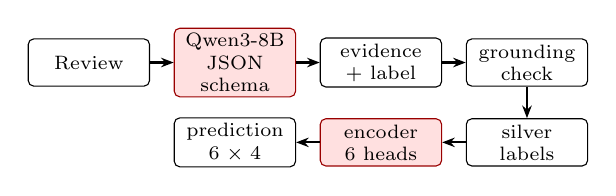
\begin{tikzpicture}[font=\scriptsize,
  box/.style={draw, rounded corners=2pt, minimum height=6mm, inner sep=2pt, align=center, text width=14mm},
  llm/.style={box, fill=red!12, draw=red!60!black},
  arr/.style={-{Stealth[length=1.6mm]}, thick}]
\node[box] (r) {Review};
\node[llm, right=3mm of r] (q) {Qwen3-8B\\JSON schema};
\node[box, right=3mm of q] (e) {evidence\\+ label};
\node[box, right=3mm of e] (g) {grounding\\check};
\node[box, below=4mm of g] (s) {silver\\labels};
\node[llm, left=3mm of s] (m) {encoder\\6 heads};
\node[box, left=3mm of m] (p) {prediction\\$6\times4$};
\foreach \u/\v in {r/q,q/e,e/g,g/s,s/m,m/p} \draw[arr] (\u) -- (\v);
\end{tikzpicture}
\caption{Labeling and training pipeline. An LLM writes an evidence phrase and a label per aspect; labels with ungrounded evidence are reset to \emph{none}; the resulting silver labels train an encoder with one four-way head per aspect.}
\label{fig:pipeline}
\end{figure}

\subsection{Task Definition}
Each review receives one label from $\{$positive, negative, neutral, none$\}$ for each of six aspects (Table~\ref{tab:aspects}). \textit{Neutral} means that the review discusses the aspect without a clear opinion, or praises and criticizes it about equally; \textit{none} means that the aspect is not discussed. A seventh aspect, pacing, was annotated with the others but is excluded from all experiments.

\begin{table}[t]
\caption{Aspects and their scope}
\label{tab:aspects}
\centering
\small
\begin{tabular}{lp{6.1cm}}
\toprule
Aspect & Covers \\
\midrule
Acting & performances, cast, casting, voice acting \\
Story & plot, script, dialogue, characters as written, twists, ending \\
Visual & cinematography, lighting, special effects, sets, costumes \\
Sound & music, score, songs, sound effects, audio quality \\
Direction & the director's work; a name alone is not enough \\
Overall & the reviewer's verdict on the film as a whole \\
\bottomrule
\end{tabular}
\end{table}

\subsection{Silver Labeling with a Local LLM}
\label{sec:labeling}
\textbf{Model and decoding.} We label every review with Qwen3-8B~\cite{qwen3} quantized to 4 bits (Q4\_K\_M, 5.0~GB) and served by llama.cpp~\cite{llamacpp} (build b12081) on the same 8~GB laptop GPU used for training. Decoding is greedy (temperature 0) with the model's reasoning mode disabled, and the output is constrained by a JSON schema, so that every response contains all aspects and only valid labels. Reviews longer than 12{,}000 characters (three reviews) are shortened to their beginning and end.

\textbf{Evidence-first prompt.} The prompt defines the labels and aspects, lists rules for hard cases (generic praise counts only for \emph{overall}; a named actor without judgment is \emph{neutral} for acting; sarcasm counts by its intended meaning; an explicit score decides \emph{overall}) and gives three short examples. For each aspect the model must first copy the shortest exact phrase (at most 20 words) in which the reviewer talks about that aspect, and only then output the label; with no such phrase, the label must be \emph{none}. After decoding, a non-\emph{none} label is reset to \emph{none} if its evidence is empty or not grounded in the review, i.e., neither a substring of the review nor covered to at least 70\% by the review's word tokens. \emph{Overall} is exempt, because a verdict can be implicit. Fig.~\ref{fig:pipeline} summarizes the pipeline.

\textbf{Prompt development.} To choose the prompt we used a reference set of 300 validation reviews (150 positive, 150 negative, random seed 2026). These reviews were labeled by a larger proprietary LLM (Claude) following the written guideline; they are therefore a stronger-model reference rather than human gold labels, and they were used only for prompt development, never for model selection or evaluation. The reference \emph{overall} labels agree with the IMDb star ratings on 99.3\% of the 95\% of reviews with a decided verdict. Table~\ref{tab:prompt} compares a label-only prompt (v2) with the evidence-first prompt (v3). The label-only prompt often assigned \emph{neutral} or \emph{negative} to aspects the review never mentions, inferring them from the overall tone; the evidence step removes most of these errors, and mean $\kappa$ rises from 0.54 to 0.72. Only story remains below 0.6.

\begin{table}[t]
\caption{Agreement of Qwen3-8B with the 300-review reference set (Cohen's $\kappa$)}
\label{tab:prompt}
\centering
\small
\setlength{\tabcolsep}{2.5pt}
\begin{tabular*}{\columnwidth}{@{\extracolsep{\fill}}lccccccc@{}}
\toprule
Prompt & Act. & Story & Vis. & Sound & Dir. & Over. & Mean \\
\midrule
v2 (label) & 0.43 & 0.57 & 0.57 & 0.39 & 0.48 & 0.77 & 0.54 \\
v3 (evidence) & 0.67 & 0.60 & 0.70 & 0.78 & 0.79 & 0.77 & \textbf{0.72} \\
\bottomrule
\end{tabular*}
\end{table}

\textbf{Cost and output.} With two parallel requests, labeling ran at 0.65 reviews per second (about 21 hours of GPU time for the corpus), with no failed request. The grounding check reset 275 of the roughly 300{,}000 non-overall labels (0.09\%), most of them for sound (105) and story (97). Every record stores the model, prompt version and hash, the evidence phrases and the reset aspects, so that the team can verify labels quickly.

\subsection{Classification Models}
All models share one architecture: an encoder reads the review, the representation of the first token passes through dropout and a linear layer with $6\times4$ outputs, and the output is reshaped into one four-way softmax per aspect. The loss is the sum over aspects of the class-weighted cross-entropy,
\begin{gather}
\mathcal{L} = \sum_{a=1}^{6} w^{(a)}_{y_a}\,\bigl(-\log p_a(y_a\mid x)\bigr),\\
w^{(a)}_c = \mathrm{clip}\Bigl(\sqrt{\tfrac{N}{4\,n^{(a)}_c}},\,0.2,\,5\Bigr),
\end{gather}
where $n^{(a)}_c$ is the number of training reviews with label $c$ for aspect $a$. The square-root weights stop the frequent \emph{none} class from dominating visual, sound and direction without overweighting the rarest classes.

Reviews longer than 512 tokens keep the first 128 and the last 382 tokens~\cite{sun2019}. This affects 12.3\% of test reviews with the BERT tokenizer and 11.8\% with the RoBERTa tokenizer. We compare three encoders:
\begin{itemize}
\item \textit{Frozen BERT + BiLSTM:} a frozen BERT-base encoder whose token states feed a BiLSTM~\cite{hochreiter1997,schuster1997} with 768 units per direction (dropout 0.5); the concatenated final states replace the first-token representation. This mirrors the model of our earlier binary study.
\item \textit{BERT-base FT:} BERT-base (uncased, 110M parameters)~\cite{devlin2019}, fully fine-tuned.
\item \textit{RoBERTa-large FT:} RoBERTa-large (355M parameters)~\cite{liu2019roberta}, fully fine-tuned with gradient checkpointing~\cite{chen2016} to fit in 8~GB.
\end{itemize}

\section{Experiments}
\label{sec:experiments}

\subsection{Data Description}
We use the 50{,}000 labeled IMDb reviews~\cite{maas2011} with the leakage-controlled split of our earlier work: the official 25{,}000-review test set (3{,}581 movies) is kept intact, 223 duplicate or leaking training reviews are removed, and the remaining training reviews are split by movie into 21{,}027 training reviews (2{,}910 movies) and 3{,}750 validation reviews (514 movies). No movie occurs in two splits. Each review also keeps its star rating (1--4 or 7--10), which the LLM never sees.

\textbf{Label distribution.} Table~\ref{tab:dist} shows the training distribution; validation and test differ from it by less than three points for every cell. Story is criticized 2.3 times more often than praised. Sound, direction and visual are not mentioned in most reviews, and neutral is rare for every aspect, which makes Macro-F1 sensitive to a few hundred neutral examples.

\begin{table}[t]
\caption{Silver label distribution on the training set (\%)}
\label{tab:dist}
\centering
\small
\begin{tabular*}{\columnwidth}{@{\extracolsep{\fill}}lrrrr@{}}
\toprule
Aspect & Positive & Negative & Neutral & None \\
\midrule
Acting & 36.7 & 29.2 & 9.1 & 25.0 \\
Story & 21.4 & 49.5 & 15.7 & 13.4 \\
Visual & 19.7 & 12.1 & 5.1 & 63.1 \\
Sound & 8.6 & 6.3 & 2.1 & 83.0 \\
Direction & 9.3 & 11.8 & 3.4 & 75.4 \\
Overall & 43.9 & 45.7 & 8.7 & 1.7 \\
\bottomrule
\end{tabular*}
\end{table}

\subsection{Experimental Setting}
\label{sec:protocol}
\textbf{Metrics.} For each aspect we compute Macro-F1 over the four labels (over the labels present in the gold or predicted labels), and the primary score is the mean over the six aspects. Two secondary metrics separate the sub-problems: \emph{detection F1} treats every non-\emph{none} label as ``mentioned,'' and \emph{sentiment Macro-F1} is computed over positive, negative and neutral on the reviews where the silver label is not \emph{none}. Because no human-labeled test set is available, all these scores are measured \emph{against the silver labels}, so they show how well each model reproduces the LLM annotator, not accuracy against human judgment.

\textbf{An LLM-independent check.} The IMDb star rating is written by the reviewer and was never shown to the LLM. For the \emph{overall} aspect we therefore also report the fraction of reviews predicted positive or negative (``decided'') and the accuracy of those predictions against the rating (positive for 7--10 stars).

\textbf{Statistical testing.} Reviews of the same movie are not independent, so we use a paired bootstrap~\cite{efron1993} that resamples the 3{,}581 test movies with replacement ($B=10{,}000$). In each resample we recompute the Macro-F1 of both systems from per-movie confusion counts, average over the three matched seeds and take the difference. We report percentile 95\% confidence intervals and two-sided $p$-values with add-one correction (floor $2\times10^{-4}$), adjusted with the Holm procedure~\cite{holm1979} separately for the three comparisons of the mean score and for the 18 per-aspect comparisons.

\textbf{Implementation details.} All use AdamW~\cite{loshchilov2019} with weight decay 0.01, linear warm-up over 10\% of the steps followed by linear decay, gradient clipping at 1.0 and BF16 autocast (Table~\ref{tab:hparams}). After each epoch we compute the mean Macro-F1 over the six aspects on the validation set and keep the best epoch; the test set is evaluated once per run. Every configuration is trained with seeds 42, 43 and 44 on a laptop RTX 5070 GPU (8~GB) with PyTorch~\cite{paszke2019} and Transformers~\cite{wolf2020}.

\begin{table}[t]
\caption{Training settings (effective batch size 32 for all)}
\label{tab:hparams}
\centering
\small
\setlength{\tabcolsep}{4pt}
\begin{tabular*}{\columnwidth}{@{\extracolsep{\fill}}lccc@{}}
\toprule
 & BiLSTM & BERT-base & RoBERTa-large \\
\midrule
Encoder & frozen & fine-tuned & fine-tuned \\
Learning rate & $3\times10^{-4}$ & $2\times10^{-5}$ & $1\times10^{-5}$ \\
Micro-batch $\times$ accum. & $16\times2$ & $8\times4$ & $4\times8$ \\
Epochs & 8 & 3 & 3 \\
Peak GPU memory & 0.9 GB & 3.6 GB & 6.3 GB \\
Training time per seed & 23 min & 15 min & 63 min \\
\bottomrule
\end{tabular*}
\end{table}

\section{Results and Discussion}
\label{sec:results}

\subsection{Main Comparison}
Table~\ref{tab:main} lists the test results. Fine-tuned RoBERTa-large reaches 74.19\% mean Macro-F1, 6.33 points above fine-tuned BERT-base and 11.61 points above the frozen BiLSTM. The ranking holds for detection and for sentiment, but the gap is much larger for sentiment (75.01\% vs.\ 62.26\%) than for detection (92.09\% vs.\ 87.71\%): finding whether an aspect is discussed is comparatively easy, while judging the opinion requires reading it in context. Run-to-run variation is small; the largest standard deviation over seeds is 0.36 points, for the frozen BiLSTM. On the star-rating check, RoBERTa-large decides 88.8\% of the reviews and agrees with the star rating on 97.5\% of them.

\begin{table}[t]
\caption{Test results against silver labels (mean $\pm$ SD over three seeds; Macro-F1 in \%)}
\label{tab:main}
\centering
\small
\setlength{\tabcolsep}{2.5pt}
\begin{tabular*}{\columnwidth}{@{\extracolsep{\fill}}lcccc@{}}
\toprule
Model & Macro-F1 & Detect. & Sentim. & Stars \\
\midrule
Frozen BiLSTM & 62.58 $\pm$ 0.36 & 87.71 & 62.26 & 94.6 \\
BERT-base FT & 67.86 $\pm$ 0.11 & 90.82 & 67.09 & 95.2 \\
RoBERTa-large FT & \textbf{74.19 $\pm$ 0.13} & \textbf{92.09} & \textbf{75.01} & \textbf{97.5} \\
\bottomrule
\multicolumn{5}{@{}p{\columnwidth}@{}}{\scriptsize Detect./Sentim.: detection F1 and sentiment Macro-F1. Frozen BiLSTM: frozen BERT-base with a BiLSTM head. Stars: accuracy of decided \emph{overall} predictions against the IMDb star rating.}
\end{tabular*}
\end{table}

\subsection{Per Aspect and Significance}
Fig.~\ref{fig:aspects} breaks the score down by aspect. RoBERTa-large is best on all six aspects, from 71.6\% on story to 77.6\% on acting. Story is the hardest aspect for every model: reviews mix plot summary with judgment, and story has the largest share of neutral labels. Table~\ref{tab:sig} shows that all three pairwise differences of the mean score are significant, with confidence intervals far from zero. The same holds for each of the 18 per-aspect comparisons (Holm-adjusted $p\le0.0036$, the floor for 18 tests); the smallest is BERT-base over the frozen BiLSTM on \emph{overall}, +3.07 points [2.21, 3.91].

\begin{figure}[t]
\centering
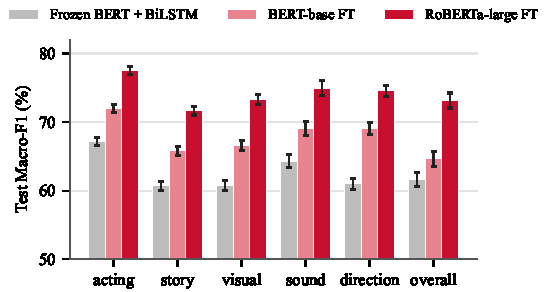
\includegraphics[width=\columnwidth]{fig_aspects}
\caption{Test Macro-F1 per aspect against silver labels (mean over three seeds). Error bars are 95\% movie-clustered bootstrap intervals.}
\label{fig:aspects}
\end{figure}

\begin{table}[t]
\caption{Paired comparisons of mean test Macro-F1 (points)}
\label{tab:sig}
\centering
\small
\begin{tabular*}{\columnwidth}{@{\extracolsep{\fill}}lcc@{}}
\toprule
Comparison & $\Delta$ & 95\% CI \\
\midrule
RoBERTa-large FT vs BERT-base FT & +6.33 & [5.99, 6.66] \\
RoBERTa-large FT vs frozen BiLSTM & +11.61 & [11.24, 11.97] \\
BERT-base FT vs frozen BiLSTM & +5.28 & [4.97, 5.59] \\
\bottomrule
\multicolumn{3}{l}{\scriptsize Holm-adjusted bootstrap $p=0.0006$ (the floor for three tests) for all rows.}
\end{tabular*}
\end{table}

\subsection{Error Analysis}
\textbf{Neutral is the weak class.} Fig.~\ref{fig:classf1} shows per-class F1 for RoBERTa-large. Positive and negative reach 75--94\%, and \emph{none} exceeds 92\% for the three rarely mentioned aspects, but neutral stays between 35.5\% (sound) and 53.5\% (overall). The larger encoder helps most exactly here: for neutral, RoBERTa-large improves on BERT-base by 9--17 points per aspect, for example from 23.5\% to 38.8\% on visual. The \emph{none} class of \emph{overall} is also weak (51.5\%), but it covers only 1.7\% of the reviews.

\begin{figure}[t]
\centering
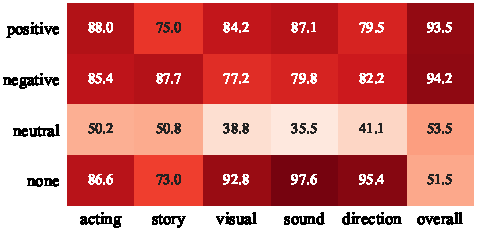
\includegraphics[width=\columnwidth]{fig_class_f1}
\caption{Per-class test F1 (\%) of RoBERTa-large for each aspect, mean over three seeds.}
\label{fig:classf1}
\end{figure}

\textbf{Detection versus polarity.} The error types differ by aspect. For visual, sound and direction, most RoBERTa-large errors are about whether the aspect is mentioned at all: 66--73\% of the errors involve \emph{none} on one side (\emph{none}$\rightarrow$negative alone accounts for 17--18\%). For acting and story, most errors involve neutral (55\% and 64\%; silver neutral predicted positive alone is 16\% of the story errors), and for \emph{overall} 78\% do. Confusions between positive and negative are rare: 2--16\% of the errors depending on the aspect.

\textbf{Long reviews.} Reviews longer than 512 tokens are clearly harder for all models: RoBERTa-large scores 75.1\% on reviews that fit and 66.8\% on those that do not; the gap is 7.4 points for BERT-base and 5.8 points for the BiLSTM. In our binary study, the same head--tail input closed this gap completely for RoBERTa-large. For aspects, an opinion about the music or the camera work can sit in the discarded middle, so a single verdict at the end of a review no longer suffices.

\textbf{Stars as a sanity check.} Fig.~\ref{fig:stars} plots RoBERTa-large's \emph{overall} prediction against the star rating. Extreme ratings are almost always predicted with the matching polarity (95.5\% negative at one star, 92.0\% positive at ten stars). Neutral predictions concentrate at the boundary ratings: 23.1\% of four-star and 22.6\% of seven-star reviews, compared with 2.1\% of one-star reviews. This pattern was not supervised by the ratings and matches what one would expect from mixed reviews, which suggests that the neutral class is meaningful even though it is hard to predict.

\begin{figure}[t]
\centering
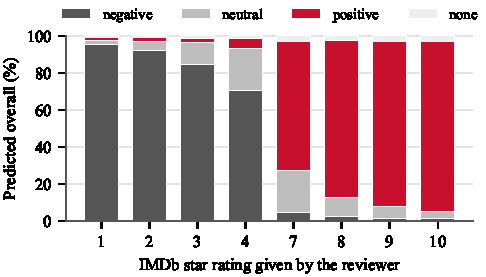
\includegraphics[width=\columnwidth]{fig_stars}
\caption{Distribution of RoBERTa-large's \emph{overall} prediction by the reviewer's IMDb star rating (test set, three seeds pooled).}
\label{fig:stars}
\end{figure}

\textbf{Consistent disagreements.} For each aspect we counted the test reviews on which all nine runs (three models, three seeds) predict the same label and that label differs from the silver one. These reviews make up 1.6\% (sound) to 6.5\% (story) of the test set, and the most frequent pattern for story is a silver \emph{neutral} that all models read as negative (369 reviews) or positive (336). Such cases are candidates for silver-label errors as well as for systematic model errors. A short inspection finds both. In one one-star review the LLM labeled \emph{overall} as neutral, quoting ``It was okay,'' although the reviewer writes this only as what they would have thought before the ending, which then explains the review's ``undeniably hostile tone''; all models predict negative, which agrees with the rating. In another, the LLM correctly labeled sound negative from the phrase ``a bad music,'' which all nine runs missed. These reviews should be prioritized in any human verification.

\subsection{Human Verification Protocol}
\label{sec:human}
Because the silver labels come from an LLM, scores against them measure agreement with that annotator, not accuracy against human judgment. We prepared, but did not carry out within the project timeline, a verification protocol for three annotators. It samples 400 test reviews stratified by star rating, with at most one review per movie (mean length 232 words). Each annotator labels 200 reviews: 100 shared by all three, used to measure inter-annotator agreement with Fleiss' $\kappa$~\cite{fleiss1971}, and 100 of their own. For shared reviews the human label is the majority vote; reviews without a majority are excluded for that aspect. The released tooling creates the annotation workbooks and computes inter-annotator $\kappa$, the agreement of the Qwen3-8B labels with the human labels, and the Macro-F1 of every trained model against them. By default annotators see the LLM label and evidence, which speeds up labeling but may anchor them toward the LLM; a blind mode hides both and gives an unbiased estimate of LLM accuracy.

Until such a verification is done, the only evidence independent of the LLM is the star-rating check of Section~\ref{sec:results}, which covers the \emph{overall} aspect only.

\subsection{Discussion}
\textbf{Cost.} The whole pipeline ran on one laptop: about 21 hours of GPU time for labeling and 5 hours for the nine training runs. Running the labeler locally was what made the project feasible, and constrained decoding removed the need for any output repair: no request failed.

\textbf{Evidence as a cheap control.} The evidence step helped in two ways. It made the LLM commit to a specific phrase, which removed most labels inferred from overall tone, and it gave annotators a direct pointer for verification. The automatic grounding check reset few labels (0.09\%); most of the gain came from the instruction itself rather than from the filter.

\subsection{Limitations}
(i) All main results are measured against silver labels, and the models are bounded by the quality of those labels; the reference set used for prompt development was itself labeled by an LLM, and no human verification of the test labels was carried out, so we cannot report accuracy against human judgment for any aspect except the star-rating check on \emph{overall}. (ii) Agreement on story ($\kappa$=0.60) is the lowest, so story results are the least reliable. (iii) The neutral class is rare and its boundary is subjective. (iv) Reviews longer than 512 tokens lose the middle part. (v) We study one corpus in one language.

\textbf{Future work.} The first step is to carry out the human verification protocol of Section~\ref{sec:human}, preferably in blind mode. Further steps are encoders that read whole reviews~\cite{beltagy2020}, aspect-specific attention that also returns evidence, filtering or re-weighting silver labels by the agreement between the LLM and the trained models, and fine-tuning on a human-verified subset.

\section{Conclusion}
\label{sec:conclusion}
We built a six-aspect sentiment dataset over all 49{,}777 reviews of a movie-grouped IMDb split by labeling it with a local 8B-parameter LLM, and showed that an evidence-first prompt with a grounding check improves agreement with a reference set from $\kappa$=0.54 to 0.72. Trained on these silver labels, a fine-tuned RoBERTa-large reaches 74.19\% mean Macro-F1, significantly ahead of BERT-base and a frozen BERT with a BiLSTM on every aspect, and its \emph{overall} predictions agree with the reviewers' star ratings on 97.5\% of decided reviews. The remaining errors are concentrated on the neutral class and on long reviews.

\section*{Author Contributions}
Ngô Ngọc Trường Sơn: idea, implementation, all experiments, analysis and writing. Vũ Quốc Đạt and Nguyễn Gia Phúc: discussion of the study design and review of the manuscript. All authors read and approved the paper.

\section*{Funding}
This research did not receive any specific grant from funding agencies in the public, commercial, or not-for-profit sectors.

\section*{Declaration of Competing Interest}
The authors declare that they have no known competing financial interests or personal relationships that could have appeared to influence the work reported in this paper.

\section*{Declaration of Generative AI and AI-Assisted Technologies}
Besides Qwen3-8B, which produced the silver labels as described in Section~\ref{sec:labeling}, AI assistants (including Claude) were used to help write and debug code, to run and check experiments and to draft and edit the text; Claude also labeled the 300-review reference set used for prompt development. The authors checked every reported number against the saved outputs and take full responsibility for the code, the results and the paper.

\section*{Acknowledgment}
We thank Maas \textit{et al.} for the IMDb dataset and the Qwen and llama.cpp teams for releasing their models and software.

\begin{thebibliography}{00}
\bibitem{maas2011} A. L. Maas, R. E. Daly, P. T. Pham, D. Huang, A. Y. Ng, and C. Potts, ``Learning word vectors for sentiment analysis,'' in \textit{Proc. 49th Annu. Meeting Assoc. Comput. Linguistics: Human Language Technologies}, Portland, OR, USA, 2011, pp. 142--150.
\bibitem{liu2019roberta} Y. Liu \textit{et al.}, ``RoBERTa: A robustly optimized BERT pretraining approach,'' arXiv:1907.11692, 2019.
\bibitem{sun2019} C. Sun, X. Qiu, Y. Xu, and X. Huang, ``How to fine-tune BERT for text classification?'' in \textit{Proc. China National Conf. Chinese Computational Linguistics (CCL)}, 2019, pp. 194--206.
\bibitem{pontiki2014} M. Pontiki, D. Galanis, J. Pavlopoulos, H. Papageorgiou, I. Androutsopoulos, and S. Manandhar, ``SemEval-2014 Task 4: Aspect based sentiment analysis,'' in \textit{Proc. 8th Int. Workshop on Semantic Evaluation (SemEval)}, 2014, pp. 27--35.
\bibitem{zhang2023survey} W. Zhang, X. Li, Y. Deng, L. Bing, and W. Lam, ``A survey on aspect-based sentiment analysis: Tasks, methods, and challenges,'' \textit{IEEE Trans. Knowl. Data Eng.}, vol. 35, no. 11, pp. 11019--11038, 2023.
\bibitem{thet2010} T. T. Thet, J.-C. Na, and C. S. G. Khoo, ``Aspect-based sentiment analysis of movie reviews on discussion boards,'' \textit{J. Information Science}, vol. 36, no. 6, pp. 823--848, 2010.
\bibitem{sun2019absa} C. Sun, L. Huang, and X. Qiu, ``Utilizing BERT for aspect-based sentiment analysis via constructing auxiliary sentence,'' in \textit{Proc. NAACL-HLT}, 2019, pp. 380--385.
\bibitem{devlin2019} J. Devlin, M.-W. Chang, K. Lee, and K. Toutanova, ``BERT: Pre-training of deep bidirectional transformers for language understanding,'' in \textit{Proc. NAACL-HLT}, 2019, pp. 4171--4186.
\bibitem{wang2021gpt3} S. Wang, Y. Liu, Y. Xu, C. Zhu, and M. Zeng, ``Want to reduce labeling cost? GPT-3 can help,'' in \textit{Findings of EMNLP}, 2021, pp. 4195--4205.
\bibitem{gilardi2023} F. Gilardi, M. Alizadeh, and M. Kubli, ``ChatGPT outperforms crowd workers for text-annotation tasks,'' \textit{Proc. Nat. Acad. Sci.}, vol. 120, no. 30, e2305016120, 2023.
\bibitem{hinton2015} G. Hinton, O. Vinyals, and J. Dean, ``Distilling the knowledge in a neural network,'' arXiv:1503.02531, 2015.
\bibitem{qwen3} A. Yang \textit{et al.}, ``Qwen3 technical report,'' arXiv:2505.09388, 2025.
\bibitem{llamacpp} G. Gerganov \textit{et al.}, ``llama.cpp: LLM inference in C/C++,'' GitHub repository, \url{https://github.com/ggml-org/llama.cpp}, 2023.
\bibitem{lowerated} Lowerated, ``imdb-reviews-rated,'' Hugging Face dataset, \url{https://huggingface.co/datasets/Lowerated/imdb-reviews-rated}.
\bibitem{hochreiter1997} S. Hochreiter and J. Schmidhuber, ``Long short-term memory,'' \textit{Neural Computation}, vol. 9, no. 8, pp. 1735--1780, 1997.
\bibitem{schuster1997} M. Schuster and K. K. Paliwal, ``Bidirectional recurrent neural networks,'' \textit{IEEE Trans. Signal Process.}, vol. 45, no. 11, pp. 2673--2681, 1997.
\bibitem{chen2016} T. Chen, B. Xu, C. Zhang, and C. Guestrin, ``Training deep nets with sublinear memory cost,'' arXiv:1604.06174, 2016.
\bibitem{loshchilov2019} I. Loshchilov and F. Hutter, ``Decoupled weight decay regularization,'' in \textit{Proc. Int. Conf. Learning Representations (ICLR)}, 2019.
\bibitem{paszke2019} A. Paszke \textit{et al.}, ``PyTorch: An imperative style, high-performance deep learning library,'' in \textit{Advances in Neural Information Processing Systems 32}, 2019.
\bibitem{wolf2020} T. Wolf \textit{et al.}, ``Transformers: State-of-the-art natural language processing,'' in \textit{Proc. EMNLP: System Demonstrations}, 2020, pp. 38--45.
\bibitem{efron1993} B. Efron and R. J. Tibshirani, \textit{An Introduction to the Bootstrap}. New York, NY, USA: Chapman \& Hall, 1993.
\bibitem{holm1979} S. Holm, ``A simple sequentially rejective multiple test procedure,'' \textit{Scandinavian J. Statistics}, vol. 6, no. 2, pp. 65--70, 1979.
\bibitem{fleiss1971} J. L. Fleiss, ``Measuring nominal scale agreement among many raters,'' \textit{Psychological Bulletin}, vol. 76, no. 5, pp. 378--382, 1971.
\bibitem{beltagy2020} I. Beltagy, M. E. Peters, and A. Cohan, ``Longformer: The long-document transformer,'' arXiv:2004.05150, 2020.
\end{thebibliography}

\end{document}

